\documentclass[12pt,a4paper]{article}
\usepackage[english]{babel}
\usepackage[utf8]{inputenc} 
\usepackage[T1]{fontenc} 
\usepackage{ae}
\usepackage{textcomp} 
\usepackage{float}
\usepackage{enumitem}
\usepackage[colorlinks=false,urlcolor=black,hidelinks]{hyperref}

%
\usepackage{fancyref}
\usepackage{fancyhdr} 
\usepackage{amsmath}
\usepackage[dvipsnames]{xcolor}
\usepackage{url}
\usepackage{makeidx}
\usepackage{listings}
\usepackage{acronym}
\usepackage{rotating}
\usepackage{tabularx}
\usepackage{multirow}
\usepackage{multirow, makecell}
\newtheorem{theorem}{Definition}
\usepackage{algcompatible}% http://ctan.org/pkg/algorithmicx
\usepackage{algpseudocode}
\usepackage[]{algorithm}
\usepackage{subcaption}

\makeatletter
\newcommand{\algcolor}[2]{%
  \hskip-\ALG@thistlm\colorbox{#1}{\parbox{\dimexpr\linewidth-2\fboxsep}{\hskip\ALG@thistlm\relax #2}}%
}
\newcommand{\algemph}[1]{\algcolor{Gray}{#1}}
\makeatother

\renewcommand{\algorithmicforall}{\textbf{for each}}
%
% PDF settings

% colorlinks=false, pdfborder={0 0 0} = keine farbigen Links
%
% Header and Footer Style
\pagestyle{fancy}
\fancyhead{}
\fancyhead[L]{\slshape\nouppercase{\rightmark}}
\fancyfoot{}
\fancyfoot[C]{\thepage}
\renewcommand{\headrulewidth}{0pt}
\renewcommand{\sectionmark}[1]{\markright{\thesection\ #1}}
%
% No identation
\setlength\headheight{15pt}
\setlength\parindent{0pt} 
%
% Custom commands
\newcommand\zb{z.\,B.\ }
\renewcommand\dh{d.\,h.\ }
\newcommand\parbig{\par\bigskip}
\newcommand\parmed{\par\medskip}
%\newcommand{\mailto}[1]{\href{mailto:#1}{#1}}
%
% C# Code Listing Style
\definecolor{darkblue}{rgb}{0,0,.6}
\definecolor{darkgreen}{rgb}{0,0.5,0}
\definecolor{darkred}{rgb}{0.5,0,0}
\lstset{language=[Sharp]C, basicstyle=\ttfamily\small\upshape, commentstyle=\color{darkgreen}\sffamily, keywordstyle=\color{darkblue}\rmfamily\bfseries, breaklines=true,tabsize=2,xleftmargin=3mm, xrightmargin=3mm,numbers=none,frame=single,stringstyle=\color{darkred},
showstringspaces=false}
%
% Titel + Author 
\title{
\includegraphics[width=0.6\textwidth]{pictures/logo}\\[3ex]
Aggregation of security attributes based on the granularity level of the system \\[3ex]
{\normalsize Thesis Submitted in Partial Fulfilment of the Requirements for the Degree of }\\[3ex]
Master of Science \\[3ex]
{\normalsize to the Department of Computer Science of Freie Universität Berlin \\ by}\\[1ex]
}

\author{\\Artemij Voskobojnikov \\
{\normalsize Student ID: 4557770 }\\
{\normalsize \href{mailto:voskobojnikov.artemij@gmail.com}{voskobojnikov.artemij@gmail.com}}\\\\
{\normalsize First Reviewer: Prof. Dr. Jörn Eichler}\\
{\normalsize Second Reviewer: Prof. Dr. Marian Margraf}\\
}

\date{Berlin, 18th of July}


\begin{document}

\begin{titlepage}

\pagenumbering{alph}
\maketitle
\thispagestyle{empty}

\vfill{}

\vfill{}

\end{titlepage}
\clearpage\pagenumbering{Roman}
% !TEX encoding = UTF-8 Unicode
\subsection*{Affirmation of independent work}
I hereby declare that I wrote this thesis myself without sources other than
those indicated herein. All parts taken from published and unpublished
scripts are indicated as such.
\parbig
Berlin, 9th of August
\\\\

\rule{120pt}{1pt}\\
(Artemij Voskobojnikov)
% !TEX encoding = UTF-8 Unicode
\pagestyle{empty}
\section*{Acronyms}
\begin{acronym}
\acro{SSA}{Software System Architecture}
\acro{SA}{Security Architecture}
\acro{ST}{Security Target}
\acro{TOE}{Target of Evaluation}
\acro{SFR}{Security Functional Requirement}
\acro{SG}{Security Goal}
\acro{UML}{Unified Modeling Language}
\acro{SUS}{System under Study}
\acro{MOF}{Meta Object Facility}
\acro{OMG}{Object Management Group}
\acro{}{}
\acro{}{}
\acro{}{}
\acro{}{}
\acro{}{}
\acro{}{}
\acro{}{}
\acro{}{}
\acro{}{}
\acro{}{}
\acro{}{}



\end{acronym}
% !TEX encoding = UTF-8 Unicode
\pagestyle{empty}
\listoffigures
% !TEX encoding = UTF-8 Unicode
\subsection*{Abstract}
\pagestyle{empty}

Computer systems have theoretical and real weaknesses that can be exploited by adversaries \cite{Pfleeger:2006:SC:1177321}. Computer security tries to protect these systems and the contained entities from adversaries.

Security models serve the purpose of depicting the system components, potential threats and countermeasures as well as connections and used data in a comprehensible manner. 

Such components can become very complex for large information systems with a significant number of components and interrelations amongst them. This complexity can result in an increased difficulty of detection of all potential impacts \cite{branagan}.

System abstraction addresses this by creating representation layers providing only relevant properties of a system. In computer security such projections could be used to focus on the security or insecurity of certain sub-systems.

Researchers proposed aggregation methods for a variety of security attributes such as security requirements \cite{Menzel2008} or vulnerabilities/exploits \cite{Noel:2004:MAG:1029208.1029225} but were either theoretical or very limited. 

Moreover is manual intervention usually needed  when creating and maintaining security concepts  which may result in incomplete or only partially available models.

This thesis proposes an approach that is not limited to a specific security attribute such as previous work. By gathering security-related information from abstraction layers with higher and lower granularities we are able to derive new security attributes that can be used for an enhanced and more thorough security assessment of a system.


\newpage
\pagestyle{empty}
\tableofcontents
\pagestyle{plain}
\clearpage\pagenumbering{arabic}
\setcounter{page}{1}
% !TEX encoding = UTF-8 Unicode
\section{Introduction}

Computer-related systems have theoretical and real weaknesses that could potentially be exploited by adversaries \cite{Pfleeger:2006:SC:1177321}. Computer security tries to protect these systems from theft or damage by unauthorized individuals. 

The system components, the potential threats and countermeasures as well as the interactions amongst them can be depicted in security models, such as a security concept (Section \ref{subsec:sec_concept}).

For large information systems such concepts can become very complex because of the number of the involved sub-systems/components. Interconnectivity and interdependence amongst components may increase the overall system complexity and therefore the difficulty of detection of all potential impacts \cite{branagan}.

Methods for system abstraction that address this problem already exist. In this thesis system abstraction is seen as the creation of representation layers providing only relevant properties of a system. This results in a better level of understanding for the respective user \cite{pohl}. 

An exemplary approach is the creation of projections that reflect different granularity levels of a system by displaying different levels of details \cite{thyssen2010system}.

In computer security such projections could be used to focus on the security or insecurity of certain sub-systems. Security attributes of components could thus be viewed separately and the security risk for a respective component could be derived. 

As already mentioned security concepts can be used to depict security attributes of a certain computer-related system and similar to many modeling practices manual intervention is needed to some degree. This may result in incomplete or only partially available models. 

For computer security this may result in missing attributes such as threats or security goals for certain granularity levels. An approach deriving new information based on the initial model would therefore be very useful.

Aggregation methods for security attributes have already been suggested by researchers, e.g. transformation rules for security requirements by Menzel et al. \cite{Menzel2008} or aggregation rules for attack graphs by Noel et al. \cite{Noel:2004:MAG:1029208.1029225}. 

None of those methods take granularity levels or general system hierarchy into account whereas the goal of this thesis is to provide an approach which makes it possible for a user to select a sub-system of interest, i.e. a projection which reflects a certain granularity level, and provides the corresponding security attributes.

The approach presented in this thesis is not limited to a specific security attribute such as security requirements (\cite{Menzel2008}) or exploits (\cite{Noel:2004:MAG:1029208.1029225}). A complete transformation rule set for security attributes in a security concept is provided and implemented.

The relevant attributes as well as dependencies and possible aggregations will be shown to ensure an overall complete picture of the selected sub-system. This information can then be used to assess and improve the security level of the selected projection or its dependencies.

\subsection{Outline of the Thesis}

Section \ref{sec:background} provides the background material for the thesis. Computer security is briefly covered and the term \textit{Security Concept} is being introduced. Section \ref{sec:related_work} covers related areas and previous approaches of security attribute aggregation as well as granularity levels and model verification. Section \ref{sec:approach} discusses the goal of the approach and the defined transformation rules and the aggregation of security attributes. Section \ref{sec:implementation} covers the technology that was used for the implementation of the previously defined transformation rules. Section \ref{sec:conclusion} concludes by outlining the contributions and identifying avenues for future work.            
% !TEX encoding = UTF-8 Unicode
%!TEX root = thesis.tex

\newpage
\section{Background}

Prior to addressing the actual approach and implementation some concepts and terms have to be introduced. Firstly, the term \textit{security concept}, as it is used throughout the thesis, is being described. A definition of \textit{granularity levels} and system abstraction follows. Lastly, a section covers \textit{model transformations} and \textit{aggregation rules} on security attributes.

\subsection{Security}
Many different definitions of security exist. Here, a slightly adapted definition of a \textit{information security management system} (ISMS), as it is found in the ISO/IEC 27001 \cite{iso27001}, is being used.
\begin{quote}
\textit{\glqq The information security management system preserves the confidentiality, integrity and availability
of information by applying a risk management process and gives confidence to interested parties that
risks are adequately managed\grqq}    
\end{quote}

It is also added that the ISMS is integrated into the overall management structure and is vital for many of the organizational processes \cite{iso27001}.

The definition above only covers information security, which in the scope of this thesis, is insufficient. Here, we define security as the preservation of confidentiality, integrity and availability of assets, where assets can be either physical or logical.

\subsection{Enterprise Security}
To define the term \textit{security concept} one has to look at the architecture of enterprises to understand the interconnectivity and interdependence between services, security being one of them. 

\subsubsection{Enterprise Architecture}

Information systems tend to be a very complex artifacts that combine different views and requirements from various stakeholders of different backgrounds \cite{alex}. 

Software, IT platforms and IT related goals in general are covered in an \textit{Information System Architecture} (ISA). ISA does not take any business-driven influences into account and is therefore insufficient when describing the complex dependencies in corporations, especially when it comes to security as described in Subsection \ref{subsec:secarch}.   

\textit{Enterprise Architecture Modeling} tries to overcome such possible difficulties and combines IT related concerns with business and organizational goals and shows possible interrelationships. It therefore provides an approach for an improved understanding of complex enterprise processes \cite{earch}. The Federal Deposit Insurance Corporation (FDIC) published the results of an audit of its own implementation of E-Government principles \cite{fdicaudit} and their division of information technology in Figure \ref{fig:fdic} depicts the interrelations very well. 

\begin{figure}[H]
\centering
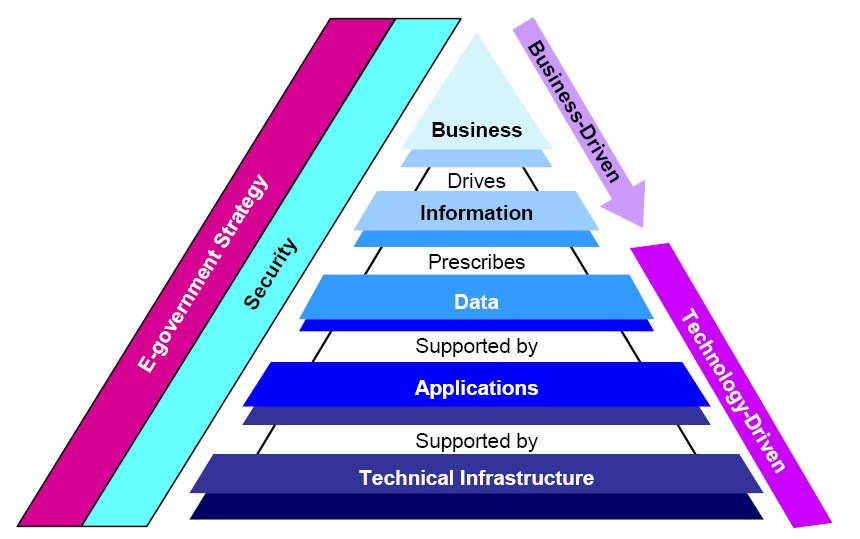
\includegraphics[width=0.75\textwidth]{pictures/fdic.jpg}
\caption{Division of Information Technology by FDIC}
\label{fig:fdic}
\end{figure}

\subsubsection{Security Architecture}
\label{subsec:secarch}

Information Security has often been merely an afterthought in corporations \cite{ansfederal} until a concept of a \textit{Security Architecture}, published in a whitepaper by The Gartner Group \cite{kreizman}, was introduced. According to \cite{kreizman} an \textit{Enterprise Information Security Architecture} (EISA) is an essential tool for improving security processes in corporations. EISA principles stand in a direct relationship with the EA principles and should be validated against them \cite{kreizman}. To highlight this relationship security considerations during phases of the \textit{The Open Group Architecture Framework Architecture Development Method} (TOGAF ADM), which is shown in Figure \ref{fig:togaf}, will be briefly described.

\begin{figure}[H]
\centering
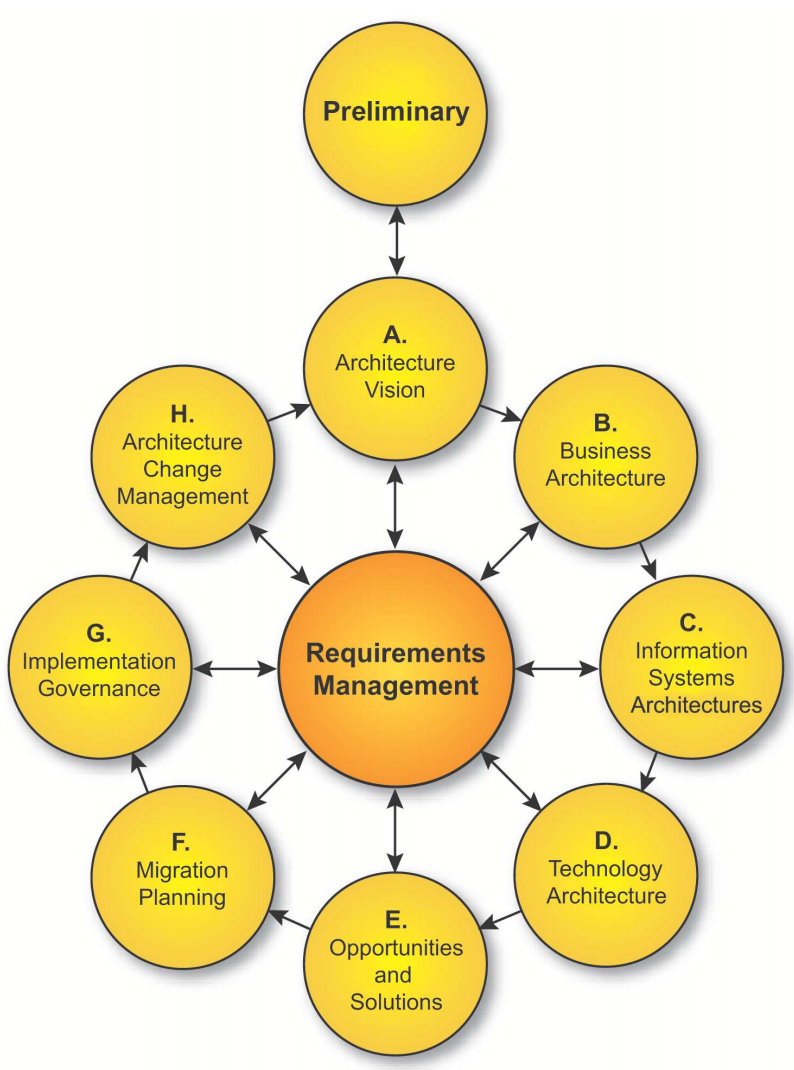
\includegraphics[width=0.6\textwidth]{pictures/togaf_overview.png}
\caption{Overview of the phases of TOGAF}
\label{fig:togaf}
\end{figure}

Security concerns can be found throughout the TOGAF phases which hints at the overall importance of security in corporations. TOGAF combines four architecture domains, the \textit{Business Architecture}, the \textit{Data Architecture}, the \textit{Application Architecture} and the \textit{Technology Architecture}. The following section will depict security considerations of two domains to show possible interrelations.

During the \textit{Business Architecture} phase in the ADM actors and handlers of the system have to be identified. Costs and potential incoveniences because of security measures have to be assessed as well. In general one can say that the impacts of security/insecurity on the business/product are being highlighted. It is tried to put an emphasis on security as early as possible to prevent costly changes in later phases in the ADM.

During the \textit{Information System Architecture} phase the classification levels of processed data have to be determined and documented. Direct dependencies to the \textit{Business Architecture} are also listed, e.g. the identification of information lifespan according to business goals and regulations. 

Similar relations can be found for security considerations from various phases of the ADM. This once again shows the overall presence of security and the high level of complexity within an enterprise.

\subsubsection{Common Criteria}
The overview of TOGAF showed the importance of security in corporations. The following section will present a way of modeling security concerns for an asset of interest.

Common Criteria proposes an evaluation by using a so called \textit{Security Target} (ST), a construct that encapsulates the \textit{Target of Evaluation} (TOE), threats to the TOE and countermeasures \cite{commoncriteria}. The goal of the evaluation is to show that the used countermeasures are sufficient to counter potential threats and thus implying that the TOE is sufficiently protected.

\begin{figure}[H]
\centering
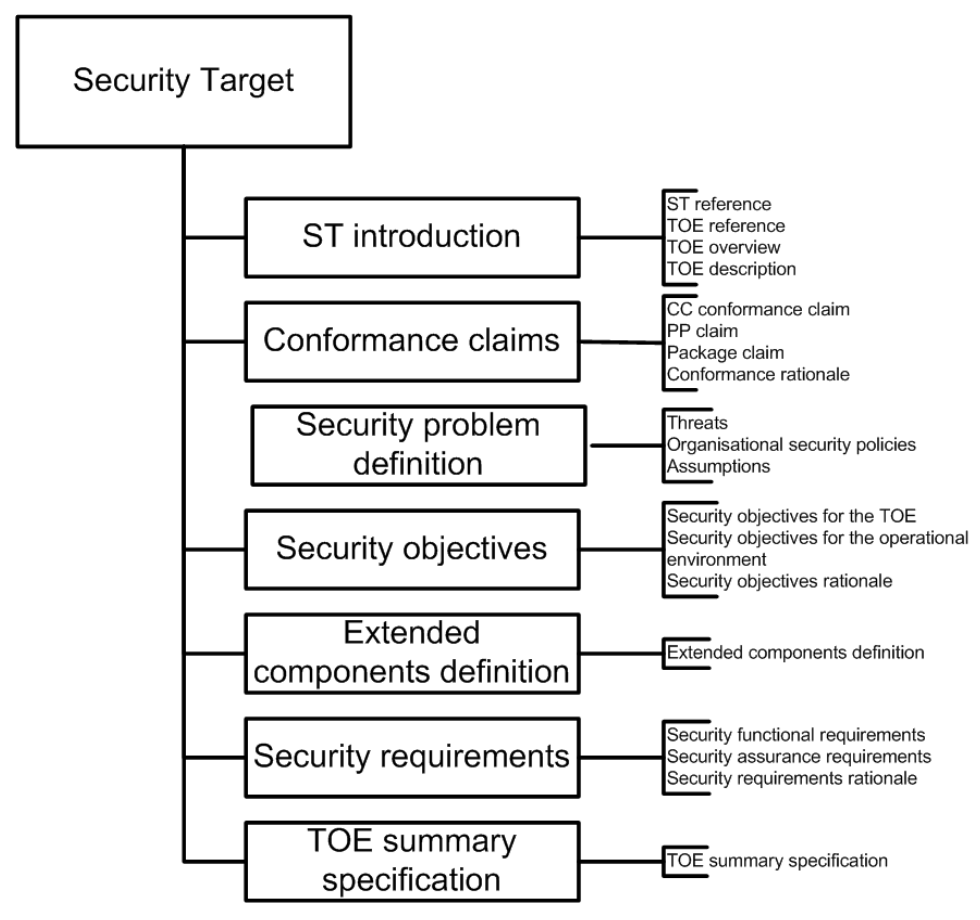
\includegraphics[width=0.85\textwidth]{pictures/sectarget.png}
\caption{Overview of the Security Target contents}
\label{fig:sectarget}
\end{figure}

A description of all the contents of a ST is unnecessary here and only the key security attributes of a ST, that will be used to construct a \textit{Security Concept} (Subsection \ref{subsubsec:secconc}), are being introduced.

The \textit{Security Problem Definition} defines, as the name suggests, the security problem that is being addressed. Apart from containing guidelines and assumptions it contains \textit{Threats} which are \textit{\glqq[...] adverse actions performed by a threat agent on an asset\grqq} (\cite{iso27001}, p. 66).

\textit{Security Objectives} is an abstract solution to the previously defined security problem. There exists a possibility to divide the \textit{Security Objectives} into part wise solutions, one being the \textit{Security Objectives for the TOE} and the other being the \textit{Security Objectives for the Operational Environment}

\subsubsection{Security Concept}
\label{subsubsec:secconc}

\subsection{Granularity Levels}

\subsection{Model Transformation}
\subsubsection{Allocation}
\subsubsection{Aggregation rules}


\bibliographystyle{plain}
\bibliography{refs}

\end{document}
